\title{POO - Classe Abstrata}

\author{Prof. Gabriel Rodrigues Caldas de Aquino}

\institute
{
    gabrielaquino@ic.ufrj.br\\
    
    Instituto de Computação -
    Universidade Federal do Rio de Janeiro % Your institution for the title page
}
\date{Compilado em: \\ \today} % Date, can be changed to a custom date

%----------------------------------------------------------------------------------------
%    PRESENTATION SLIDES
%----------------------------------------------------------------------------------------

%------------------------------------------------
\section{Revisão Inicial}
%------------------------------------------------

\begin{frame}
    % Print the title page as the first slide
    \titlepage
\end{frame}
%------------------------------------------------




\begin{frame}{Classes Abstratas na POO}
    Um componente do desenvolvimento moderno de software é a 
    \textbf{Programação Orientada a Objetos (POO)}, 
    que permite organizar o código de forma 
    \textbf{escalável}, \textbf{modular} e \textbf{reutilizável}. 
    
    \vspace{0.3cm}
    As \textbf{classes abstratas} são um dos conceitos centrais da POO, 
    fundamentais para criar um \textbf{modelo} (template) que outras classes podem usar.

\begin{block}{Pergunta}
    O que vocês acham que é uma classe abstrata?
\end{block}
\end{frame}


\begin{frame}{Classe Abstrata em POO}

\begin{block}{Definição}
\begin{itemize}
    \item Uma \textbf{classe abstrata} é uma classe que não pode ser instanciada diretamente.
    \item Atua apenas como base (superclasse) para outras classes.
    \item Pode conter:
    \begin{itemize}
        \item \textbf{Métodos implementados}: já possuem código definido.
        \item \textbf{Métodos abstratos}: devem obrigatoriamente ser sobrescritos nas subclasses concretas.
    \end{itemize}
\end{itemize}
\end{block}

\begin{block}{Objetivo}
Garantir que certas operações sejam obrigatoriamente implementadas pelas subclasses, definindo uma interface comum.
\end{block}

\end{frame}

\begin{frame}{O que é uma Classe Abstrata?}
    Uma \textbf{classe abstrata} é como um \textbf{molde} (ou \textbf{template}) para outras classes.  
    Ela define métodos que devem estar presentes em qualquer classe que herde dela, 
    mas não fornece o código específico desses métodos.
    
    \vspace{0.3cm}
    Pense nela como um \textbf{esqueleto mas sem dizer como preencher o resto}.
\end{frame}


\begin{frame}{Por que usar Classes Abstratas?}
    \begin{itemize}
        \item Definem um \textbf{molde} para outras classes.
        \item Obrigam a implementação de métodos específicos nas subclasses.
        \item Melhoram a \textbf{organização} e a \textbf{reutilização} do código.
        \item Permitem \textbf{polimorfismo}, ou seja, diferentes objetos 
              compartilhando uma interface comum.
    \end{itemize}
\end{frame}


\begin{frame}{Exemplo de Classe Abstrata}
    Suponha que você está construindo um programa para calcular a área de diferentes formas geométricas.

    \begin{itemize}
        \item Você cria uma \textbf{classe abstrata} chamada \texttt{Forma}, que define que toda forma deve ter um método \texttt{area()}.
        \item Mas \texttt{Forma} não especifica como \texttt{area()} funciona, pois a fórmula depende do tipo de forma.
        \item Cada forma específica (como \texttt{Circulo} ou \texttt{Retangulo}) herda de \texttt{Forma} e fornece sua própria implementação de \texttt{area()}.
    \end{itemize}
\end{frame}

\begin{frame}[fragile]{Antes das Classes Abstratas}

\small
\begin{verbatim}
class Forma:
    pass
    def area(self):
      pass
class Retangulo(Forma):
    def __init__(self, largura, altura):
        self.largura = largura
        self.altura = altura
    def area(self):
        return self.largura * self.altura
class Circulo(Forma):
    def __init__(self, raio):
        self.raio = raio
    def area(self):
        import math
        return 3.14 * self.raio**2
\end{verbatim}

\end{frame}

\begin{frame}[fragile]{Depois das classes abstratas}

\small
\begin{verbatim}
from abc import ABC, abstractmethod
# Classe abstrata
class Forma(ABC):
    @abstractmethod
    def area(self):
        pass
    @abstractmethod
    def perimetro(self):
        pass
# Subclasse concreta
class Circulo(Forma):
    def __init__(self, raio):
        self.raio = raio
    def area(self):
        return 3.14159 * self.raio ** 2
    def perimetro(self):
        return 2 * 3.14159 * self.raio
\end{verbatim}

\end{frame}

\begin{frame}[fragile]{Exemplo Completo de Classe Abstrata}
\small
\begin{columns}[T]

\begin{column}{0.48\textwidth}
\begin{verbatim}
from abc import ABC, abstractmethod
class Forma(ABC):
    @abstractmethod
    def area(self):
        pass
    @abstractmethod
    def perimetro(self):
        pass
class Circulo(Forma):
    def __init__(self, raio):
        self.raio = raio
    def area(self):
        return 3.14159 * self.raio ** 2
    def perimetro(self):
        return 2 * 3.14159 * self.raio
\end{verbatim}
\end{column}

\begin{column}{0.48\textwidth}
\begin{verbatim}
class Retangulo(Forma):
    def __init__(self, largura,
    altura):
        self.largura = largura
        self.altura = altura

    def area(self):
        return self.largura
        * self.altura

    def perimetro(self):
        return 2 * (self.largura
        + self.altura)
\end{verbatim}
\end{column}

\end{columns}
\end{frame}



\begin{frame}{Por que usar Classes Abstratas em Python?}

As classes abstratas são úteis quando queremos:

\begin{itemize}
    \item \textbf{Garantir a implementação de métodos}: os métodos abstratos funcionam como um \textbf{contrato}, exigindo que cada subclasse forneça sua própria implementação, evitando inconsistências.
    \item \textbf{Estimular a reutilização de código}: classes abstratas podem ter métodos concretos que reduzem duplicação e promovem o princípio DRY (\textit{Do Not Repeat Yourself}).
    \item \textbf{Melhorar legibilidade e manutenibilidade}: fornecem uma estrutura consistente e transparente, facilitando a compreensão e manutenção do código.
    \item \textbf{Permitir polimorfismo}: possibilitam escrever código genérico que funciona com diferentes subclasses, aumentando a extensibilidade e adaptabilidade do software.
\end{itemize}

\end{frame}



\begin{frame}{Passos para Criar e Usar Classes Abstratas em Python}

\begin{enumerate}
    \item Importar \texttt{ABC} e \texttt{abstractmethod} do módulo \texttt{abc}.
    \item Definir a classe abstrata como subclasse de \texttt{ABC}.
    \item Definir métodos abstratos usando o decorador \texttt{@abstractmethod}.
    \item Sobrescrever os métodos abstratos nas subclasses não abstratas.
\end{enumerate}

\begin{block}{Objetivo}
Garantir que todas as subclasses concretas implementem os métodos essenciais definidos na classe abstrata, criando uma interface comum.
\end{block}

\end{frame}

\begin{frame}{Como o módulo abc garante a implementação de métodos}
\begin{itemize}
    \item Qualquer subclasse de uma classe abstrata deve implementar todos os métodos decorados com \texttt{@abstractmethod}.
    \item Se uma subclasse não implementar todos os métodos abstratos, Python impede sua instanciação.
    \item Um \texttt{TypeError} é gerado, ajudando a identificar falhas de implementação cedo.
    \item Isso garante que todas as subclasses concretas sigam o comportamento e design esperados da classe abstrata.
\end{itemize}
\end{frame}

\begin{frame}{Especificação da classe abstrata Animal}
    \begin{figure}
        \centering
        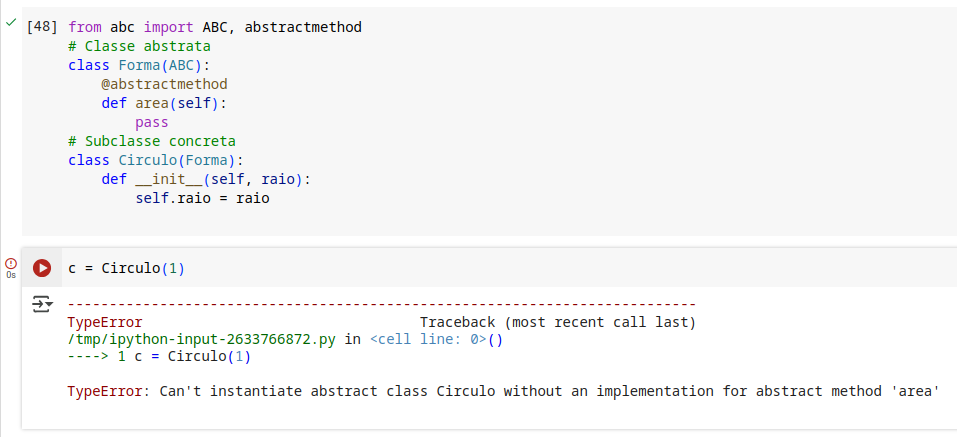
\includegraphics[width=\linewidth]{Images/classe-abstrata-erro.png}

        \label{fig:placeholder}
    \end{figure}
\end{frame}


\begin{frame}[fragile]{Exemplo: Erro ao não implementar métodos abstratos}
\small
\begin{verbatim}
class Retangulo(Forma):
    def __init__(self, largura, altura):
        self.largura = largura
        self.altura = altura

    # Métodos area() e perimetro() não implementados

# Tentativa de instanciar
r = Retangulo(5, 10)
# TypeError:
# Can't instantiate abstract class Retangulo
# with abstract methods area, perimetro
\end{verbatim}
\end{frame}


\begin{frame}{Resumo do Módulo ABC}
    O módulo \textbf{abc} oferece suporte nativo para classes abstratas.  
    \begin{itemize}
        \item "ABC" significa \textbf{Abstract Base Classes}.
        \item Fornece ferramentas como a classe \texttt{ABC} e o decorador \texttt{@abstractmethod}.
        \item Permite definir métodos abstratos que obrigam a implementação nas subclasses.
        \item Possibilita implementar um esqueleto de funcionalidades comuns.

    \end{itemize}
\end{frame}



\begin{frame}[fragile]{Classe Abstrata: Papel do \texttt{@abstractmethod}}

\begin{block}{Função do \texttt{@abstractmethod}}
\begin{itemize}
    \item Indica que o método é \textbf{abstrato} e deve ser implementado em subclasses concretas.
    \item Garante que todas as subclasses forneçam sua própria implementação.
    \item Permite que a classe abstrata defina uma \textbf{interface comum}.
\end{itemize}
\end{block}

\begin{block}{Consequência}
Se uma subclasse de \texttt{Animal} não implementar \texttt{emitir\_som()}, o Python gera um erro de instância:  
\texttt{TypeError: Can't instantiate abstract class X with abstract methods emitir\_som}
\end{block}




\end{frame}

\begin{frame}{Especificação da classe abstrata Animal}
    \begin{figure}
        \centering
        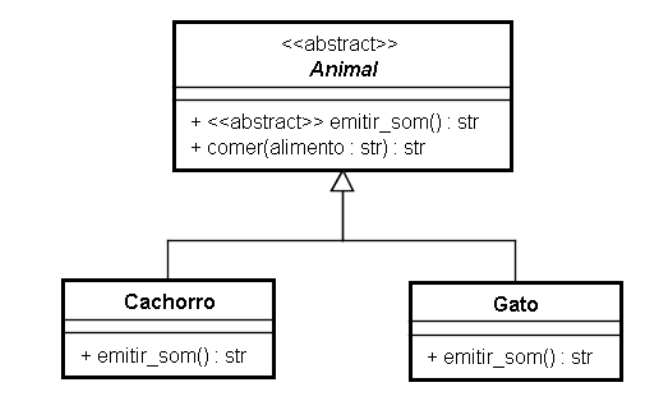
\includegraphics[width=0.5\linewidth]{Images/classe-abstrata-animal.png}

        \label{fig:placeholder}
    \end{figure}
\end{frame}

%-----------------------------------
\begin{frame}[fragile]{Classe Abstrata: Animais - Definição}
\small
\begin{verbatim}
from abc import ABC, abstractmethod
class Animal(ABC):
    def __init__(self, nome):
        self.nome = nome
    @abstractmethod
    def emitir_som(self):
        pass
class Cachorro(Animal):
    def emitir_som(self):
        print(f"{self.nome} faz Au Au!")
class Gato(Animal):
    def emitir_som(self):
        print(f"{self.nome} faz Miau!")
class Pato(Animal):
    def emitir_som(self):
        print(f"{self.nome} faz Arrrww!")
\end{verbatim}

\end{frame}

%-----------------------------------
\begin{frame}[fragile]{Classe Abstrata: Animais - Uso e Saída}

\begin{verbatim}
c = Cachorro("Rex")
g = Gato("Mimi")
p = Pato("Donald")

c.emitir_som()  # Rex faz Au Au!
g.emitir_som()  # Mimi faz Miau!
p.emitir_som()  # Donald faz Arrrww!
\end{verbatim}

\begin{block}{Saída Esperada}
Rex faz Au Au! \\
Mimi faz Miau! \\
Donald faz Arrrww!
\end{block}

\end{frame}
